
\documentclass[10pt,letterpaper]{article}
\usepackage[utf8]{inputenc}
\usepackage{amsmath}
\usepackage{amsfonts}
\usepackage{amssymb}
\usepackage{graphicx}
\author{Brock Ellefson}
\begin{document}
Policy Analysis Workflow Memo: 5 points, DUE: 4/6 
\\
\textbf{TO:}\\ Jenny Lavey\\
\textbf{FROM:}\\
      Kyle Melton (Computer Science)\\
      Brock Ellefson (Computer Science)\\
      Grace Walkuski (Computer Science)\\
      Matthew Nitschke (Computer Science)\\
      Xiaohan Zhang (English)\\
          
\section*{Proposal for Policy Analysis: Suicide Prevention Plans in Montana Schools}
\section*{Subject Description and Purpose Overview}
Suicide is a serious issue for Montana. As of 2015 we are ranked 3rd in suicide rates,  with males committing suicide four times as often than females, but females attempting suicide three times as often than their male counterparts. Suicides in Montana can be averted if schools can provide proper suicide prevention training to staff. This policy will give teachers the needed education to to assist potentially suicidal students in a healthy, safe manner.\\
\\
Our team's objective is to create an analysis and explain why it's important to prevent youth suicide and how how a proper suicide prevention plan in school can benefit our schools, our community, and our state.

\section*{Rationale} 
Suicides directly impact the wellbeing our citizens in both emotional and monetary ways. From a financial standpoint, an average each suicide costs the Montana taxpayers \$1,116,213 due to medical and work loss. That is a total of \$253,380,000 in 2010 alone. Suicide is a leading cause of death in Montana, even beating out homicide. The rate in this state is so high that on average, someone commits suicide every 32 hours. What is even more astonishing is that it is even a huge impact on the upcoming generations. Suicide is the second leading cause of death of people between the ages of 10-44. Clearly this needs to be addressed. Suicide being a major reason of death for people in this age group clearly reflects a poor method of educating children about suicide, suicide prevention, and counseling.  This policy will provide much needed, free suicide prevention education to teachers and students who interact with potential suicidal behavior on a daily basis.\\ 
\\
Statistics: https://afsp.org/about-suicide/suicide-statistics/ 

\section*{Goals}

-Explore different suicide prevention education resources \\
-Expose the harsh truths of suicide in Montana and brainstorm how to reduce this extreme rates\\
-Discover the best resources for local schools \\
-Analyze how the resources will affect its target audience\\
-How a decreased suicide rate can benefit the community\\

\section*{Methods}

Montana House Bill 374 requires the Department of Public Instruction to create free suicide prevention training resources. We will be reviewing and analyzing both this bill and the resources created by the Department of Public Instruction. Along with this analyzation, we will interview Tricia Williamson, a guidance counselor at Bozeman High, to gain better insight into Montana's suicide problem.


\section*{Individual Member Participation}

Chart of member name and responsible portion of the written analysis:
Title Page (see page 392, Keywords
Abstract (see page 392)
Table of Contents (see pages 393-394)
Summary (see pages 191-192)
Discussion (or body section) that includes: Introduction, Main Body (you determine the headings here), Conclusion, Recommendations, and References (see the example on page 193-204).
Appendices: Include your Policy Analysis Workflow Memo


\newpage
\section*{Projected Meeting Schedule}
\begin{figure}[h]
		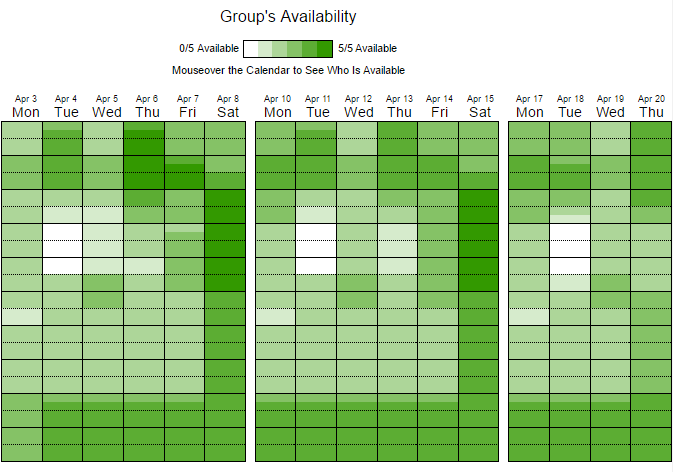
\includegraphics[scale = .5]{groupaval.png}
  		\label{fig:aval}
	\end{figure}

\section*{Tentative Outline of Analysis}

\section*{Bibliography}

Press, AMY BETH HANSON Associated. "Bill would require schools to set suicide prevention plans."\\ Bozeman Daily Chronicle. N.p., 27 Mar. 2017. Web. 04 Apr. 2017.\\
\\
http://opi.mt.gov/Programs/HealthTopics/SuicideAware.html \\
http://opi.mt.gov/pdf/Health/SuicideAware/HB374TrainingGuidance.pdf \\
http://store.samhsa.gov/shin/content//SMA12-4669/SMA12-4669.pdf \\
https://afsp.org/about-suicide/suicide-statistics/ \\
\end{document}